\documentclass{article}\usepackage[]{graphicx}\usepackage[]{color}
%% maxwidth is the original width if it is less than linewidth
%% otherwise use linewidth (to make sure the graphics do not exceed the margin)
\makeatletter
\def\maxwidth{ %
  \ifdim\Gin@nat@width>\linewidth
    \linewidth
  \else
    \Gin@nat@width
  \fi
}
\makeatother

\definecolor{fgcolor}{rgb}{0.345, 0.345, 0.345}
\newcommand{\hlnum}[1]{\textcolor[rgb]{0.686,0.059,0.569}{#1}}%
\newcommand{\hlstr}[1]{\textcolor[rgb]{0.192,0.494,0.8}{#1}}%
\newcommand{\hlcom}[1]{\textcolor[rgb]{0.678,0.584,0.686}{\textit{#1}}}%
\newcommand{\hlopt}[1]{\textcolor[rgb]{0,0,0}{#1}}%
\newcommand{\hlstd}[1]{\textcolor[rgb]{0.345,0.345,0.345}{#1}}%
\newcommand{\hlkwa}[1]{\textcolor[rgb]{0.161,0.373,0.58}{\textbf{#1}}}%
\newcommand{\hlkwb}[1]{\textcolor[rgb]{0.69,0.353,0.396}{#1}}%
\newcommand{\hlkwc}[1]{\textcolor[rgb]{0.333,0.667,0.333}{#1}}%
\newcommand{\hlkwd}[1]{\textcolor[rgb]{0.737,0.353,0.396}{\textbf{#1}}}%
\let\hlipl\hlkwb

\usepackage{framed}
\makeatletter
\newenvironment{kframe}{%
 \def\at@end@of@kframe{}%
 \ifinner\ifhmode%
  \def\at@end@of@kframe{\end{minipage}}%
  \begin{minipage}{\columnwidth}%
 \fi\fi%
 \def\FrameCommand##1{\hskip\@totalleftmargin \hskip-\fboxsep
 \colorbox{shadecolor}{##1}\hskip-\fboxsep
     % There is no \\@totalrightmargin, so:
     \hskip-\linewidth \hskip-\@totalleftmargin \hskip\columnwidth}%
 \MakeFramed {\advance\hsize-\width
   \@totalleftmargin\z@ \linewidth\hsize
   \@setminipage}}%
 {\par\unskip\endMakeFramed%
 \at@end@of@kframe}
\makeatother

\definecolor{shadecolor}{rgb}{.97, .97, .97}
\definecolor{messagecolor}{rgb}{0, 0, 0}
\definecolor{warningcolor}{rgb}{1, 0, 1}
\definecolor{errorcolor}{rgb}{1, 0, 0}
\newenvironment{knitrout}{}{} % an empty environment to be redefined in TeX

\usepackage{alltt}
\usepackage{natbib}




\IfFileExists{upquote.sty}{\usepackage{upquote}}{}
\begin{document}
\title{Franz Kafka's The Metamorphosis}
\author{Chris Kozak}
\maketitle

\begin{abstract}
\noindent In this article, we'll do some basic sentiment analysis. We're going to construct a wordcloud for Franz Kafka's The Metamorphosis. This is one of Kafka's most well-known stories.\footnote{The short story was first published in German in 1915. Many translations exist, but we'll be using the 2002 version by David Wyllie}.
\end{abstract}

\section{Packages}
 First, we've already loaded the following packages: dplyr for querying, tidytext and text mining (tm) for working with text, gutenbergr for downloading open-source books, wordcloud for generating visualizations, and knitr for compiling documents from R Markdown, Sweave and various other formats.

\begin{knitrout}
\definecolor{shadecolor}{rgb}{0.969, 0.969, 0.969}\color{fgcolor}\begin{kframe}
\begin{alltt}
\hlkwd{get_sentiments}\hlstd{(}\hlstr{'nrc'}\hlstd{)}
\end{alltt}
\begin{verbatim}
## # A tibble: 13,901 x 2
##           word sentiment
##          <chr>     <chr>
##  1      abacus     trust
##  2     abandon      fear
##  3     abandon  negative
##  4     abandon   sadness
##  5   abandoned     anger
##  6   abandoned      fear
##  7   abandoned  negative
##  8   abandoned   sadness
##  9 abandonment     anger
## 10 abandonment      fear
## # ... with 13,891 more rows
\end{verbatim}
\end{kframe}
\end{knitrout}


\section{Downloading The Metamorphosis}
For this exercise, we'll be working with Franz Kafka's The Metamorphosis, and strictly comparing the amount of joy in the book to the amount of fear. In this book, a young man turns into a giant cockroach. His family at first tries to take care of him, then get sick of taking care of him, and sick of the burdens that his metamorphosis has imposed on the family, and let him die.

\begin{knitrout}
\definecolor{shadecolor}{rgb}{0.969, 0.969, 0.969}\color{fgcolor}\begin{kframe}
\begin{alltt}
\hlstd{metamorphosis} \hlkwb{<-} \hlkwd{gutenberg_download}\hlstd{(}\hlnum{5200}\hlstd{)}

\hlstd{metamorphosis_words} \hlkwb{<-} \hlstd{metamorphosis} \hlopt
  \hlkwd{unnest_tokens}\hlstd{(word, text)}
\end{alltt}
\end{kframe}
\end{knitrout}

\noindent Word is the name of the new column we're making with the unnest_tokens command

\section{Quantifying Fear and Joy}
Next, we'll be using the tidytext package to quantify sentiment. The tidytext package comes with several built-in sentiment lexicons, including bind and AFINN, which assign values to words based on their perceived positive or negative values. But for this exercise, we will focus on the NRC emotion lexicon. This assigns words based on the seven primary emotions: joy, sadness, fear, anger, disgust, surprise, and trust. For this exercise, we only want two emotions: joy and fear.

\section{Fear}

For the next step, we will get only the fear words from metamorphosis. As Kafka's story involves a cockroach, there should be quite a few. The following commands will create a new dataframe that contains only the fear words from the NRC sentiment lexicon, and then join those words with the ones found in The Metamorphosis.

\begin{knitrout}
\definecolor{shadecolor}{rgb}{0.969, 0.969, 0.969}\color{fgcolor}\begin{kframe}
\begin{alltt}
\hlstd{nrc_fear} \hlkwb{<-} \hlkwd{get_sentiments}\hlstd{(}\hlstr{'nrc'}\hlstd{)} \hlopt
  \hlkwd{filter}\hlstd{(sentiment} \hlopt{==} \hlstr{"fear"}\hlstd{)}

\hlstd{metamorphosis_fear_words}\hlkwb{<-}\hlkwd{inner_join}\hlstd{(nrc_fear,metamorphosis_words)}
\end{alltt}
\end{kframe}
\end{knitrout}

\section{Fear in the Metamorphosis}

Next, we'll see how many unique fear words we have, and how what kind of words they are using the dim() and head() commands from R:

\begin{knitrout}
\definecolor{shadecolor}{rgb}{0.969, 0.969, 0.969}\color{fgcolor}\begin{kframe}
\begin{alltt}
\hlkwd{dim}\hlstd{(metamorphosis_fear_words)[}\hlnum{1}\hlstd{]}
\end{alltt}
\begin{verbatim}
## [1] 271
\end{verbatim}
\begin{alltt}
\hlkwd{head}\hlstd{(metamorphosis_fear_words}\hlopt{$}\hlstd{word,}\hlkwc{n}\hlstd{=}\hlnum{20}\hlstd{)}
\end{alltt}
\begin{verbatim}
##  [1] "abandoned" "abandoned" "accused"   "afraid"    "afraid"   
##  [6] "afraid"    "alarm"     "alarm"     "alarm"     "alarm"    
## [11] "alarm"     "alarm"     "anxiety"   "anxious"   "attack"   
## [16] "attack"    "austere"   "avoid"     "avoid"     "avoid"
\end{verbatim}
\end{kframe}
\end{knitrout}

\noindent This shows that The Metamorphosis has 271 words expressing fear, and lists some examples above.


\section{Fear Wordcloud}

\begin{knitrout}
\definecolor{shadecolor}{rgb}{0.969, 0.969, 0.969}\color{fgcolor}\begin{kframe}
\begin{alltt}
\hlkwd{wordcloud}\hlstd{(metamorphosis_fear_words}\hlopt{$}\hlstd{word,}
          \hlkwc{colors} \hlstd{=} \hlkwd{c}\hlstd{(}\hlstr{"red"}\hlstd{,}\hlstr{"black"}\hlstd{,}\hlstr{"gray20"}\hlstd{,}
                     \hlstr{"indianred4"}\hlstd{,}\hlstr{"tomato4"}\hlstd{))}
\end{alltt}
\end{kframe}
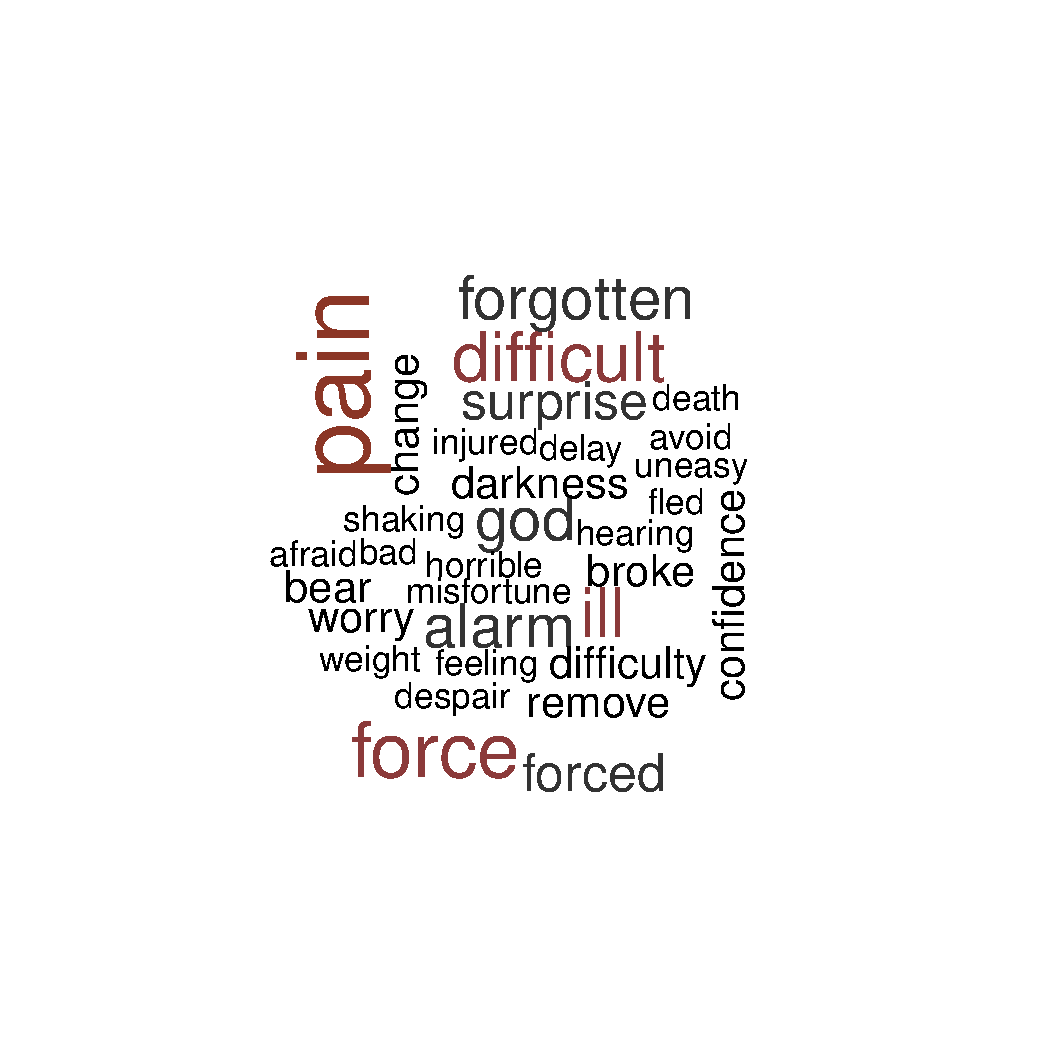
\includegraphics[width=\maxwidth]{figure/unnamed-chunk-7-1} 

\end{knitrout}


\section{Joy}
And now, we will do the same thing for the joy words from The Metamorphosis.

\begin{knitrout}
\definecolor{shadecolor}{rgb}{0.969, 0.969, 0.969}\color{fgcolor}\begin{kframe}
\begin{alltt}
\hlstd{nrc_joy} \hlkwb{<-} \hlkwd{get_sentiments}\hlstd{(}\hlstr{'nrc'}\hlstd{)} \hlopt
  \hlkwd{filter}\hlstd{(sentiment} \hlopt{==} \hlstr{"joy"}\hlstd{)}

\hlstd{metamorphosis_joy_words}\hlkwb{<-}\hlkwd{inner_join}\hlstd{(nrc_joy,metamorphosis_words)}
\end{alltt}
\end{kframe}
\end{knitrout}

\section{Joy in The Metamorphosis}

\begin{knitrout}
\definecolor{shadecolor}{rgb}{0.969, 0.969, 0.969}\color{fgcolor}\begin{kframe}
\begin{alltt}
\hlkwd{dim}\hlstd{(metamorphosis_joy_words)[}\hlnum{1}\hlstd{]}
\end{alltt}
\begin{verbatim}
## [1] 344
\end{verbatim}
\begin{alltt}
\hlkwd{head}\hlstd{(metamorphosis_joy_words}\hlopt{$}\hlstd{word,} \hlkwc{n}\hlstd{=}\hlnum{20}\hlstd{)}
\end{alltt}
\begin{verbatim}
##  [1] "affection"    "appreciation" "beautiful"    "beautiful"   
##  [5] "beer"         "captivate"    "cash"         "cash"        
##  [9] "cheer"        "child"        "child"        "child"       
## [13] "clean"        "clean"        "clean"        "comfort"     
## [17] "confidence"   "confidence"   "confidence"   "confidence"
\end{verbatim}
\end{kframe}
\end{knitrout}

\section{Joy Wordcloud}
We can see from the dimension - or dim() - command, that there are 344 unique words expressing joy in The Metamorphosis. Beer is one of them. Ironically, it features more unique words expressing joy than fear. Finally, we will generate a wordcloud to display the most common words of joy.

\begin{knitrout}
\definecolor{shadecolor}{rgb}{0.969, 0.969, 0.969}\color{fgcolor}\begin{kframe}
\begin{alltt}
\hlkwd{wordcloud}\hlstd{(metamorphosis_joy_words}\hlopt{$}\hlstd{word,}
          \hlkwc{colors} \hlstd{=}\hlkwd{c}\hlstd{(}\hlstr{"black"}\hlstd{,}\hlstr{"blue"}\hlstd{,}\hlstr{"darkcyan"}\hlstd{,}
                    \hlstr{"darkolivegreen"}\hlstd{,}\hlstr{"aquamarine3"}\hlstd{))}
\end{alltt}
\end{kframe}
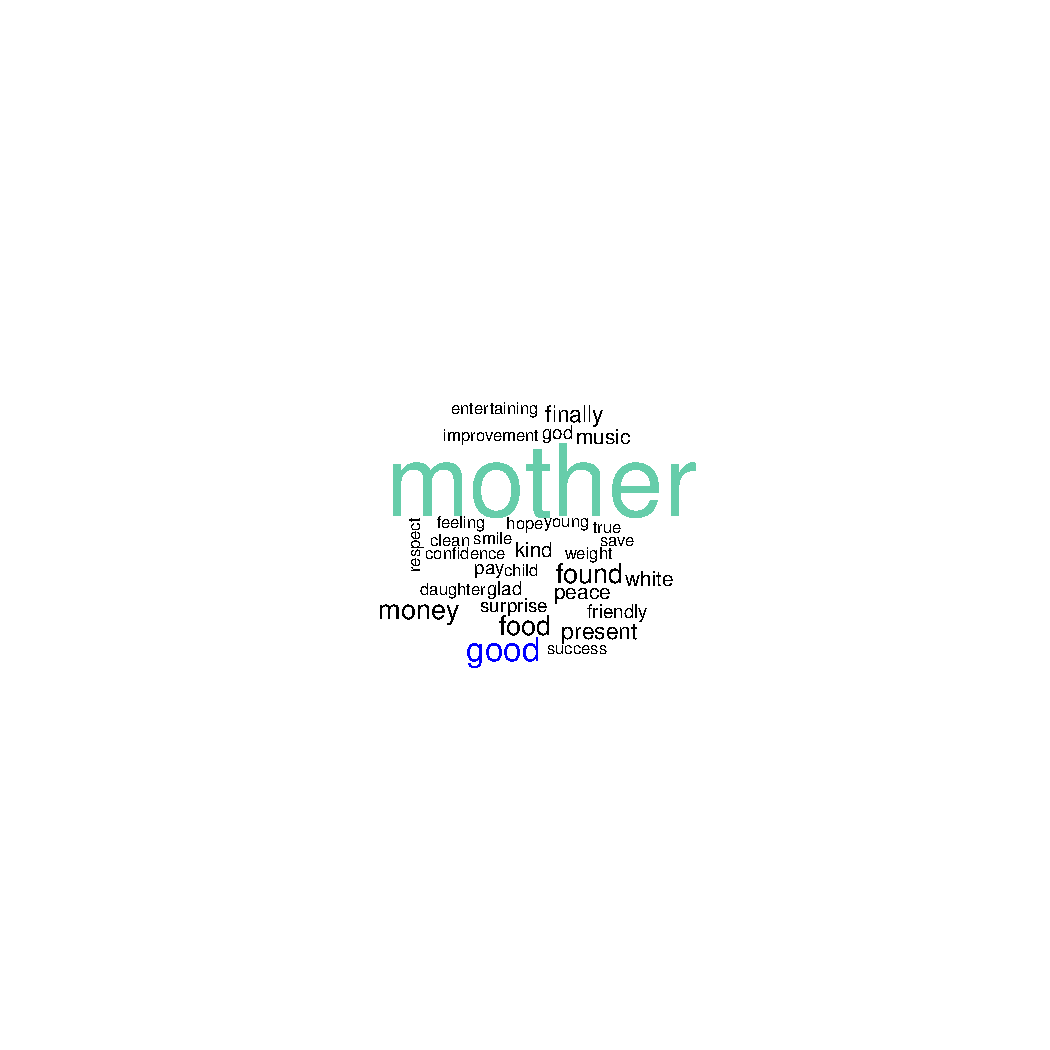
\includegraphics[width=\maxwidth]{figure/unnamed-chunk-10-1} 

\end{knitrout}

\bibliographystyle{apa}
\bibliography{source,packages}
\nocite{*}

\end{document}
